\documentclass[10pt, pscyr,nonums]{hedlabwork}
\usepackage[russian]{babel}
\usepackage[root]{hedmaths}
\usepackage{graphicx}
\graphicspath{{images/}, {plots/}}
    
\newgeometry{top=1.5cm, bottom=1.5cm, left=1cm, right=1cm}

\student{Чечеткин И. А., Ф-469}
\date{02.10.2013}
\labnum{501}
\labname{Определение постоянной Стефана-Больцмана
при помощи оптического пирометра}

\begin{document}
  \makeheader

  \emph{Цель работы:} изучение законов теплового излучения и
  экспериментальное определение постоянной Стефана-Больцмана при помощи
  оптического пирометра.
  
  \emph{Используемые при расчетах формулы и значения:}
  \( S = 2,\!3\cdot10^{-5}~\text{м}^2; \ \sigma = \cfrac{JU}{S(T^4 - T_0^4)};
  \ T = t + 273 \).

  \begin{figure}[h!]
    \center
    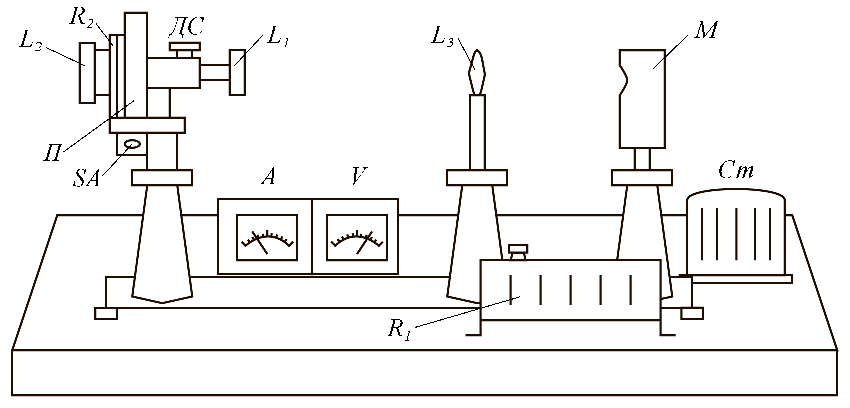
\includegraphics[width=.4\textwidth]{appearance} \hspace*{2em}
    
\includegraphics[width=.4\textwidth]{scheme} \\[.5em]
    \parbox{.4\textwidth}{\caption{Внешний вид установки}} \hspace*{2em}
    \parbox{.4\textwidth}{\caption{Принципиальная схема}}
  \end{figure}
  \vspace*{-2em}
  
  \begin{table}[h!]
    \center \caption{Результаты измерений и вычислений постоянной
    Стефана-Больцмана}
    \begin{tabular}{|C{.08}|*{4}{C{.07}|}C{.05}|C{.08}|*{2}{C{.1}|}} \hline
      \multicolumn{5}{|c|}{Температура} &
        \multirow{3}{*}{Ток \( J \)} &
        \multirow{2}{*}{Напря-} &
        \multirow{3}{*}{\( \sigma \)} &
        \multirow{3}{*}{\( \midnum{\sigma} \)} \\ \cline{1-5}
      яркостная \( t_s \) & истинная \( t \) &
        истинная \( T \) & воздуха \( t_0 \) &
        воздуха \( T_0 \) &&
        жение \( U \) && \\ \hline
      \( \vphantom{C}^{\circ}\!C \) &
        \( \vphantom{C}^{\circ}\!C \) &
        \( K \) & \( \vphantom{C}^{\circ}\!C \) &
        \( K \) & \( A \) & \( B \) &
        \( \cfrac{10^{-8} \text{Вт}}{\text{м}^2K^4} \) &
        \vspace*{.15em}\( \cfrac{10^{-8}\text{Вт}}{\text{м}^2K^4} \)
        \\[.5em] \hline
      1200 & 1283 & 1556 &
        \multirow{6}{*}{22}  &
        \multirow{6}{*}{295} &
        2,5 & 3,55 & \( 6,\!59 \pm 3,\!41 \) &
        \multirow{6}{*}{\( 8,26 \pm 3,\!71 \)} \\
      1300 & 1394 & 1667 &&& 3,0 & 4,40 & \( 7,\!44 \pm 3,\!58 \) & \\
      1400 & 1508 & 1781 &&& 3,6 & 5,55 & \( 8,\!64 \pm 3,\!89 \) & \\
      1500 & 1621 & 1894 &&& 4,2 & 6,82 & \( 9,\!68 \pm 4,\!10 \) & \\
      1600 & 1736 & 2009 &&& 4,5 & 7,45 & \( 8,\!95 \pm 3,\!57 \) & \\
      1700 & 1851 & 2124 &&&
        ---\!---\!--- & ---\!---\!--- & ---\!---\!--- & \\ \hline
    \end{tabular}
  \end{table}
  
  \emph{Подсчет погрешности} производился по формуле
  \[
    \Delta\sigma = \sqrt{\left( \pder{\sigma}{J}\Delta J \right)^2 +
    \left( \pder{\sigma}{U}\Delta U \right)^2 +
    \left( \pder{\sigma}{T}\Delta T \right)^2 +
    \left( \pder{\sigma}{T_0}\Delta T_0 \right)^2},
  \]
  где \( \Delta J = 0,\!1 \), \( \Delta U = 0,\!05 \), \( \Delta T = 200 \),
  \( \Delta T_0 = 1 \), а производные:
  \[
    \pder{\sigma}{J} = \frac{U}{S(T^4 - T_0^4)}, \ 
    \pder{\sigma}{U} = \frac{J}{S(T^4 - T_0^4)}, \ 
    \pder{\sigma}{T} = -\frac{JU}{S(T^4 - T_0^4)^2}\cdot 4T^3, \ 
    \pder{\sigma}{T_0} = \frac{JU}{S(T^4 - T_0^4)^2}\cdot 4T_0^3.
  \]
  
  \emph{Вывод:} в ходе лабораторной работы была определена постоянная
    Стефана-Больцмана при помощи оптического пирометра. В результате обработки
    полученных данных была выявлена большая относительная погрешность
    (\( \sim 45\% \)). Это может быть связано с индивидуальной восприимчивостью
    глазом яркости нити пирометра и конуса.
\end{document}
